\section{Detector por Produto Interno utilizando Análise de Compomentes Principais (IPD-B-PCA)}

Entende-se por Análise de Componentes Principais (do inglês \textit{Principal Component Analysis} - PCA), também conhecida como  Transformada de \textit{Karhunen-Loève} \cite{schurmann1996pattern}, o procedimento matemático que faz uso de transformação ortogonal para o problema de redução de dimensionalidade. A ideia central dessa técnica é, dado um conjunto de  variáveis em um sistema de coordenadas qualquer representá-lo em outro (diferente) de forma a obter, com um menor número de combinações lineares (componentes principais), um maior número possível de informações contidas nas variáveis originais. Essa técnica também é utilizada em reconhecimento de padrões \cite{waldir2010facial}, e será utilizada no projeto dos classificadores com intuito de aumentar a sua robustez.

\begin{figure}[!htb]
\centering
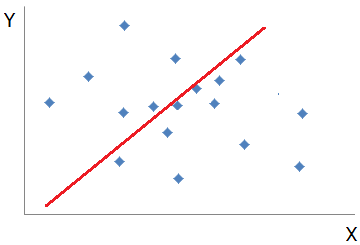
\includegraphics[scale=1]{figuras/pca.PNG}
\caption{Representação da Análise de Componentes Principais.}
\label{fig_pca}
\end{figure}

Conforme pode ser obervado na Figura \ref{fig_pca}, temos \textit{N} variáveis das quais desejamos extrair um número desejado de compontes principais. O PCA propõe uma projeção ortogonal de um vetor em um subespaço linear de menor dimensão que o original, de modo que a variância desse vetor seja a máxima possível. Matematicamente o PCA pode ser obtido da seguinte forma: Supondo um variável aleatória $\mathcal{X}_{N\text{x}1}$ com \textit{N} realizações iguais aos vetores $x_i$ a base do subespaço que possui a maior variância, definida como $\Phi  = \{ {\phi _1},...,\,{\phi _N}\}$, é obtida através da diagonalização da matriz de covariância $\sum\mathcal{X}$, onde são calculados os seus autovalores:

\begin{equation}\label{eq_autovalores}
\Lambda  = {\Phi ^{*t}}\sum\mathcal{X} \Phi
\end{equation}

onde o sobrescrito $^{*t}$ indica o transposto conjugado da matriz e $\sum \mathcal{X}$ é a matriz de covariância de $\mathcal{X}$ com média igual a zero.

\begin{figure}[!htb]
\centering
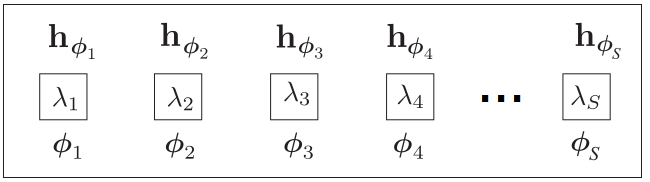
\includegraphics[scale=0.7]{figuras/esquema_Matriz.png}
\caption{\textit{N} Detectores por produto interno considerando-se \textit{N} componentes principais.}
\label{fig_esquemaMatriz}
\end{figure}

Para o nosso sistema a base $\Phi  = [{\phi _1},\,...,\,{\phi _N}]$ são os \textit{Eigenpoints}, ou seja, blocos ${\mathcal{X}_i}$ que representam características salientes da face humana denominados pontos fiduciais (em inglês, \textit{fiducial point}), conforme pode ser observado na Figura \ref{fig_esquemaMatriz}. A diagonal principal da matriz $\Lambda$ (${\lambda _1},\,...,\,{\lambda _N}$) correspondem aos autovetores da Equação \eqref{eq_autovalores}. Os autovetores são derivadas da matriz de covariância. A matriz de covariância de $\mathcal{X}$ é dada por:

\begin{equation}\label{eq_MatrizDeCovariancia}
\sum {_X = \frac{1}{{M - 1}}X{X^{*t}}}
\end{equation}

Onde  $\mathcal{X}$ é uma matriz formada por M vetores, com M>N (sendo M o número de realizações da variável aleatória $\mathcal{X}_{N\text{x}1}$) da seguinte forma:

\begin{equation}\label{eq_MatrizX}
X = [{x_1} - {\mu _x},...,{x_M} - {\mu _x}]
\end{equation}

Onde $\mu_x$ é dado por:

\begin{equation}\label{eq_mi}
{\mu _x} = \frac{1}{M}\sum\limits_{i = 1}^M {{x_i}}
\end{equation}

Tendo em vista as equações apresentadas bem como o esquema observado na Figura \ref{fig_esquemaMatriz}, faz-se necessário discriminar os autovalores $\phi$ e rejeitar os demais, tendo em vista que se trata de pontos fora da região de interesse. Com o intuito de melhor classificar essas componentes separou-se em três classes distintas, são elas: $\mathcal{A}_1$, $\mathcal{A}_2$ e $\mathcal{B}$, onde:

\begin{description}
  \item[$\bullet$ $\mathcal{A}_1$] Refere-se a classe dos componentes que desejamos detectar ($\mathcal{A}_1=\phi$)
  \item[$\bullet$ $\mathcal{A}_2$] Será formada por deslocamentos lineares de $\phi_i$
  \item[$\bullet$ $\mathcal{B}$] Essa classe comporta todas as outras componentes ($\phi_j$)
\end{description}

Utilizando-se a Equação \eqref{vetorH_final} para se determinar o detector por produto interno aplicada às componentes principais temos:

\begin{equation}\label{eq_ipd_b_pca}
h{\phi _i} = {\{ {p_1}{R_{A1}} + {p_2}{R_{A2}} + p(B){R_B}\} ^{ - 1}}\,{p_1}{\mu _{A1}}
\end{equation}

Se reescrevermos a Equação \eqref{eq_ipd_b_pca} em função dos elementos típicos das classes $\mathcal{A}_1$, $\mathcal{A}_2$ e $\mathcal{B}$ temos:

\begin{equation} \label{eq_IPD-B-PCA_Final}
h{\phi _i} = {\left\{ \begin{array}{l}
{p_1}{\phi _i}{({\phi _i})^{*t}} + {p_2}\frac{1}{{{{(2L + 1)}^2} - 1}}\,\sum\limits_{n =  - L\hfill\atop
n \ne 0\hfill}^L {\sum\limits_{m =  - L\hfill\atop
m \ne 0\hfill}^L {{\phi _i}^{(n,m)}{\phi _i}^{{{(n,m)}^{*t}}}} } \\
 + p(B)\,\frac{1}{{N - 1}}\,\sum\limits_{j = 1\hfill\atop
j \ne i\hfill}^N {{\phi _j}{{({\phi _j})}^{*t}}} 
\end{array} \right\}^{ - 1}}\,{p_1}{\phi _i}
\end{equation}

Por fim, temos que a Equação \eqref{eq_IPD-B-PCA_Final} expressa o detector por produto interno utilizando análise de componentes principais proposto.
